\section{Diseño}

\subsection{Convertidor Forward}

Se listan a continuación las especificaciones acordadas con la cátedra para el prototipo.

\begin{itemize}
    \item Tensión de entrada: $V_s=36V$
    \item Tensión de salida: $V_o=12.6V$
    \item Ciclo de trabajo mínimo: $D_{min}=0$
    \item Ciclo de trabajo máximo: $D_{max}=0.5$
    \item Frecuencia de conmutación: $f=125kHz$
    \item Corriente media en la carga: $I_{med}=1A$
\end{itemize}

Se desea obtener una variación en la corriente del inductor $\Delta i_L=25\%$ y un ripple de tensión en la salida $\Delta v=0.2\%$.
En consecuencia:

$$ \Delta i_L=I_{med}\frac{\delta i[\%]}{100}=1A\times\frac{25}{100}=0.25A $$

$$ \Delta V_o=V_{o_{med}}\times\frac{\Delta v[\%]}{100}=12.6V\times\frac{0.2}{100}=0.025V $$

En principio se dimensiona el filtro de salida compuesto por el inductor y el capacitor. 
En base a la variación de la corriente en el inductor se calcula la inductancia.
Para el ciclo de trabajo mínimo se obtiene la inductancia máxima:

$$ L=\frac{V_o(1-D)}{f\Delta i_L}=\frac{12.6V\times(1-0)}{125kHz\times0.25A}=400uH $$

En base a la ecuación de la tensión de rizado pico a pico en la salida se calcula la capacidad.
Para el ciclo de trabajo mínimo se obtiene la capacidad máxima:

$$ C=\frac{(1-D)V_o}{8\times L\times\Delta V_o\times f^2}=\frac{(1-0)\times12.6V}{8\times400uH\times0.025V\times(125kHz)^2}=10uF $$

Los dispositivos semiconductores fueron elegidos en base a su disponibilidad en el ATEI,
comprobando que puedan ser utilizados en el prototipo con los parámetros especificados en sus hojas de datos.  

Se eligieron diodos rectificadores para alta frecuencia modelo UF4007 \cite{uf4007}. 
Presenta tiempo de recuperación inversa ultra rápido, una baja caída de tensión directa, alta capacidad de sobretensión, bajas pérdidas de conmutación y alta eficiencia.
Sus características principales son: 

\begin{itemize}
    \item Máxima corriente rectificada directa promedio: $I_f=1A$
    \item Voltaje inverso pico repetitivo máximo: $V_{rrm}=1000V$
    \item Tiempo máximo de recuperación inversa: $t_{rr}=75ns$
    \item Tensión directa instantánea máxima: $V_f=1.7V$
\end{itemize}

Para los transistores se eligieron MOSFETs para switching de alta velocidad modelo IRF840 \cite{IRF840}. 
Sus características principales son: 

\begin{itemize}
    \item $P_{max}=125W$
    \item $V_{ds_{max}}=500V$
    \item $V_{gs_{max}}=20V$
    \item $I_{d_{max}}=8A$
    \item $I_{d_{repetitiva max}}=32A$
\end{itemize}

\subsection{Transformador}

La potencia aparente del transformador $P_{t}$ es la suma de la potencia de entrada $P_{i}$ y la potencia de salida $P_{o}$:

$$ P_{t}=P_{i}+P_{o}=\frac{P_{o}}{\eta}+P_{o}=\left(1+\frac{1}{\eta}\right)P_{o} $$

La tensión en el bobinado primario está dada por: 

$$ V_{1}=K_{t} f N_{1} \phi_{m} $$

donde $f$ es la frecuencia de conmutación de la señal de entrada y 
$K_t$ es un factor que vale $4.44$ si la forma de onda es sinusoidal o $4$ si es rectangular.

El flujo máximo $\phi_{m}$ se relaciona con el área de la sección transversal de la trayectoria del flujo $A_{e}$ y la densidad de flujo máxima $B_{m}$ de la siguiente manera:

$$ \phi_{m}=B_{m} \times A_{e} $$

La densidad de corriente $J$ es:

$$ J=K_jA_p^x $$

donde $K_j$ y $x$ son constantes que dependen del núcleo magnético dadas por la tabla \ref{tabla:Kj}:

\begin{table}[]
    \begin{tabular}{lcccc}
        \hline
        Tipo de núcleo   & $K_j @ 25^{\circ} C$ & $K_j @ 50^{\circ} C$ & $x$   & Pérdidas en el núcleo \\ \hline
        Pot core         & 433                  & 632                  & -0.17 & $P_{cu}=P_{fe}$       \\
        Power core       & 403                  & 590                  & -0.12 & $P_{cu}\gg P_{fe}$    \\
        E-laminated core & 366                  & 534                  & -0.14 & $P_{cu}=P_{fe}$       \\
        C-core           & 323                  & 468                  & -0.14 & $P_{cu}=P_{fe}$       \\
        Single-coil      & 395                  & 569                  & -0.14 & $P_{cu}\gg P_{fe}$    \\
        Tape-wound core  & 250                  & 365                  & -0.13 & $P_{cu}=P_{fe}$       \\ \hline
    \end{tabular}
    \caption{Valores de $K_j$ y $x$ para distintos tipos de núcleo}
    \label{tabla:Kj}
\end{table}

El factor $A_{p}$ se puede calcular como: 

$$ A_{p}=\left(\frac{P_{t} \times 10^{4}}{K_{t} f B_{m} K_{u} K_{j}}\right)^{\frac{1}{1+x}} {cm}^{4} $$

donde $K_u$ es el factor de relleno que varía entre 0.4 y 0.6 y $B_m$ es la densidad de flujo máxima.

La cantidad de alambre de cobre y la cantidad de material del núcleo (por lo general ferrita de hierro) determinan la capacidad de potencia del transformador. 
Existen distintos tipos de núcleo como toroidal, pot, power, E-laminated, EI, C, single-coil, tape-wound, etc. 
En este proyecto se trabajará con los núcleos disponibles provistos por la cátedra: E70, E42 y E30 \cite{trafos}. 

Las especificaciones obtenidas por simulación son las siguientes:
\begin{itemize}
    \item Frecuencia de la forma de onda rectangular: $f=125kHz$ y $K_{t}=4$
    \item Tensión máxima aplicada a la bobina del primario: $V_{1_{max}}=350V$ \footnote{El transformador fue diseñado antes de reemplazar el rectificador de entrada por una fuente regulable de 36V, por lo que quedó sobredimensionado.}
    \item Tensión de salida en el secundario: $V_{0}=12.6V$
    \item Corriente de salida en el secundario: $I_{0}=1A$
    \item Eficiencia: $n=95\%$
\end{itemize}

\subsubsection{Cálculos}

Potencia de salida:

$$ P_{o}=V_{o}\times I_{o}=12.6W $$

Potencia aparente: 

$$ P_t=P_o+P_i=P_o\times\left(1+\frac{1}{n}\right)=25.86W  $$

%INSERTAR IMÁGEN B-H DE KIKE!
\begin{figure}[ht]
    \centering
    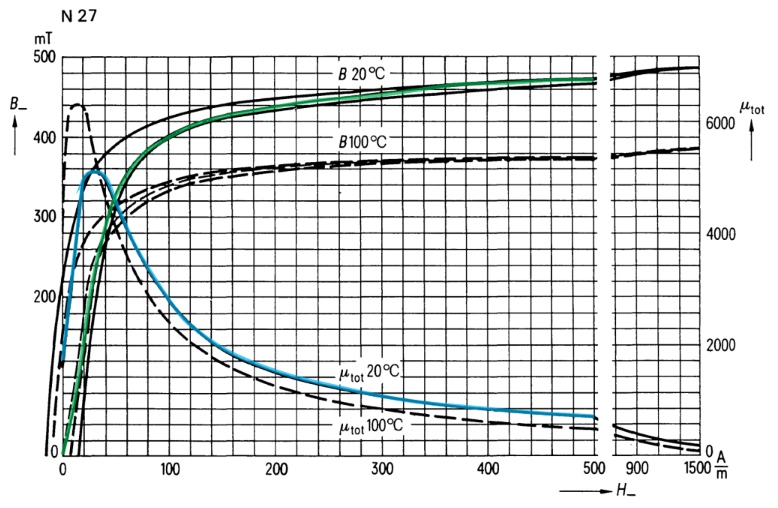
\includegraphics[width=0.8\textwidth]{images/diseno-trafos-kike/tabla_bh_kike.png}
    \caption{Gráfica B vs. H para núcleos N27}
    \label{fig:grafica-b-h}
\end{figure}

En base a las curvas de magnetización se observa como las ferrites no soportan tanto flujo como el hierro y como disminuye la permeabilidad para campos mayores.  
Presenta el ciclo de histéresis y comienza a saturar en $B=300mT$. 
La saturación implica mayor circulación de corriente que conlleva a que el núcleo deje de responder. 
Esta se da en campos menores si la temperatura aumenta con el funcionamiento del dispositivo. 
Por lo tanto se elige una inducción magnética máxima de $B_{m}=100mT$ para estar lejos del codo y asegurarnos tener la permeabilidad especificada en las hojas de datos. 

Para el núcleo E70, el área efectiva es: 

$$ A_{e}=279{mm}^{2} $$

Número de vueltas del primario:

$$ N_{1}=\frac{V_{1_{max}}}{K_{t}\times f\times B_{m}\times A_{e}}=25.09\simeq 25 $$

Número de vueltas del secundario: 

$$ N_{2}=N_{1}\times\frac{V_{2}}{V_{1}} $$

Como no se requiere ni desea elevar o reducir la tensión del secundario, se elige una relación de vueltas 1:1. 
Por lo tanto, el número de vueltas del bobinado secundario es igual al del primario. \footnote{El número de vueltas del secundario se duplicó respecto al diseño original ya que al realizar las mediciones en la PCB, la tensión del secundario era mucho menor a la simulada.}

$$ N_{2}=25 $$

A partir de la tabla \ref{tabla:Kj}, para el núcleo tipo E: $ K_{j}=366$ , $x=-0.14$ y $Pfe=Pcu$. 

Tomando el factor de relleno $K_u=0.4$:

$$ A_{p}=\left(\frac{25.86\times 10^{4}}{4\times 125kHz\times 100mT\times 0.4\times 366}\right)^{\frac{1}{1-0.14}} {cm}^4=0.0205 {cm}^4$$

La densidad de corriente resulta:

$$ J=366\times 0.0205^{-0.14} \frac{A}{cm^2}=630.7 \frac{A}{cm^2} $$

La corriente que circula por el primario es:

$$ I_1=\frac{(P_t-P_0)}{V_1}=\frac{(25.86W-12.6W)}{350V}=0.0379A $$

El área de la sección transversal del alambre desnudo del primario resulta:

$$ A_{wp}=\frac{I_1}{J}=\frac{0.0379A}{630.7 \frac{A}{cm^2}}=0.06cm^2 \times10^{-3} $$

La corriente que circula por el secundario es la corriente de salida, 
por lo tanto el área de la sección transversal del alambre desnudo del secundario resulta:

$$ A_{ws}=\frac{I_o}{J}=\frac{1A}{630.7 \frac{A}{cm^2}}=1.6cm^2\times10^{-3} $$

% AGREGAR IMÁGEN DE TABLA y COMPLETAR TEXTO DE ABAJO
\begin{table}[H]
    \centering
    \begin{tabular}{ccc}
        \hline
                   & Área                  & Resistencia          \\ \cline{2-3} 
        Tamaño AWG & $[cm^2\times10^{-3}]$ & $[10^{-6}\Omega/cm]$ \\ \hline
        10         & 52.61                 & 32.70                \\
        11         & 41.68                 & 41.37                \\
        12         & 33.08                 & 52.09                \\
        13         & 26.26                 & 65.64                \\
        14         & 20.82                 & 82.80                \\
        15         & 16.51                 & 104.3                \\
        16         & 13.07                 & 131.8                \\
        17         & 10.39                 & 165.8                \\
        18         & 8.228                 & 209.5                \\
        19         & 6.531                 & 263.9                \\
        20         & 5.188                 & 332.3                \\
        21         & 4.116                 & 418.9                \\
        22         & 3.243                 & 531.4                \\
        23         & 2.588                 & 666.0                \\
        24         & 2.047                 & 842.1                \\
        25         & 1.623                 & 1062.0               \\
        26         & 1.280                 & 1345.0               \\
        27         & 1.021                 & 1687.6               \\
        28         & 0.8046                & 2142.7               \\
        29         & 0.6470                & 2664.3               \\
        30         & 0.5067                & 3402.2               \\
        31         & 0.4013                & 4294.6               \\
        32         & 0.3242                & 5314.9               \\
        33         & 0.2554                & 6748.6               \\
        34         & 0.2011                & 3572.8               \\ \hline
        \end{tabular}
    \caption{Tabla de valores AWG}
    \label{table:awg}
\end{table}
% texto

Dado que la mayor área es $A_{ws}$, la cual es superior a la mínima, a partir de la tabla \ref{table:awg} de tamaños de cable AWG se debería utilizar el AWG 25.
Sin embargo, en base a la disponibilidad se construyeron ambos bobinados con un AWG 21. 
Sus parámetros principales son:

\begin{itemize}
    \item Diámetro del cable: $d=0.723mm$
    \item Área de la sección transversal: $A_{w}=4.116\times10^{-3}cm^2$
    \item Conductividad del cobre: $\sigma=\frac{481.9\mu\Omega}{cm}$
    \item Permeabilidad magnética del cobre: $\mu_r\simeq1$
\end{itemize}

En corriente continua, la densidad de corriente es similar en todo el conductor, pero en corriente alterna se observa que hay una mayor densidad de corriente en la superficie que en el centro. 
Este fenómeno se conoce como efecto pelicular\cite{skin} y provoca una variación de la resistencia eléctrica de un conductor en corriente alterna debido al cambio de la frecuencia $f$ de la corriente eléctrica que circula por el mismo.
Por lo tanto, para corriente alterna la mayor parte de la corriente eléctrica fluye entre la superficie y la profundidad superficial de los conductores $\delta$.
Esta última depende de la frecuencia de la corriente y de las propiedades eléctricas y magnéticas del conductor.

$$ \delta=\sqrt{\frac{1}{\pi f\mu\sigma}}=\sqrt{\frac{1}{\pi\times125kHz\times1\times4\pi\times10^{-7}\times\frac{481.9\mu\Omega}{cm}}}=65mm $$

El diámetro mínimo del conductor resulta:

$$ d_{min}=2\times\delta=130mm$$

Por lo tanto, se verifica que el diámetro del cable AWG 21 es mayor al mínimo requerido. 

Para el carrete del núcleo E70, la longitud promedio de una vuelta es: 

$$ l_{mt}=9.7cm $$

La resistencia del bobinado primario y secundario y sus pérdidas en el cobre resultan:

$$ R_p=R_s=l_{mt}\times N_{1}\times\sigma=9.7cm \times25 \times\frac{481.9\mu\Omega}{cm}=100m\Omega $$

$$ P_p=I_1^2R_p=146\mu W $$

$$ P_s=I_o^2R_s=100mW $$

En base a la tabla \ref{tabla:Kj} para un núcleo tipo E las pérdidas en el núcleo son iguales a las del cobre:

$$ P_{fe}=P_p+P_s \simeq P_s=100mW $$

La eficiencia del transformador resulta:

$$ \eta=\frac{P_o}{P_o+P_p+P_s+P_{fe}}=0.9841 (98.41\%) $$

Por lo tanto, se comprueba que la eficiencia es superior a la especificada del 95\%.  

\subsection{Inductor}

Se utiliza para almacenar energía y permitir su transferencia hacia la carga. 
Por el inductor circula una corriente continua la cual no puede ser muy elevada para evitar saturar al núcleo magnético. 

Especificaciones: 

\begin{itemize}
    \item Inductancia: $L_x=400\mu H$
    \item Corriente continua: $I_{dc}=1A$
\end{itemize}

Procedimiento de diseño \cite{diseno-trafo-kike}:

\begin{enumerate}
\item{Cálculo de la energía que debe almacenar el inductor}
$$ E=0.5\times L\times I_{dc}^2=200\mu HA^2 $$
\item{Elección del tamaño del núcleo}

En base a la disponibilidad se elige un E42/15 con material magnético N27. 
Sus parámetros son:

\begin{itemize}
    \item Longitud efectiva: $l_e=67mm$
    \item Área efectiva: $A_e=60{mm}^2$
    \item $A_l=1800nH$ y $u_e=1600$ ($gap=0mm$)
    \item $A_l=630nH$ y $u_e=562$ ($gap=0.1mm$)
    \item $A_l=400nH$ y $u_e=353$ ($gap=0.18mm$)
    \item $A_l=200nH$ y $u_e=179$ ($gap=0.34mm$)
\end{itemize}

\item{Verificar energía almacenada}

Se debe corroborar que la energía que puede almacenar el inductor sin entrehierro sea suficiente.

Con $B_m=100mT$:
$$ E_{singap}=\frac{0.5\times B_m^2\times {volumen}}{u_0\times u_e}=\frac{0.5\times B_m^2\times A_e\times l_e}{u_0\times u_e}=10\mu HA^2 $$

Con $B_m=200mT$:
$$ E_{singap}=\frac{0.5\times B_m^2\times {volumen}}{u_0\times u_e}=\frac{0.5\times B_m^2\times A_e\times l_e}{u_0\times u_e}=40\mu HA^2 $$

En ambos casos es menor a la energía que debe almacenar el inductor por lo que se evidencia la necesidad de incluir un entrehierro. 

\item{Dimensionar el entrehierro}

El entrehierro $l_0$ debe almacenar la energía $E$ con $B_{max}=100mT$.
En caso de ser necesario puede llevarse a $B_{max}=200mT$ sin problema. 

Con $B_m=100mT$:
$$ l_0=\frac{2\times E\times u_0}{A_e\times B_m^2}=0.84mm $$

Con $B_m=200mT$:
$$ l_0=\frac{2\times E\times u_0}{A_e\times B_m^2}=0.2mm $$

El gap real necesario $g$ con un núcleo tipo E es la mitad de $l_0$.

Con $B_m=100mT$:
$$ g=\frac{l_0}{2}=0.42mm $$

Con $B_m=200mT$:
$$ g=\frac{l_0}{2}=0.1mm $$

\item{Dimensionar el número de vueltas}

Se calcula el número de vueltas $N$ necesario para conseguir la inductancia $L_x$ requerida.

Con $B_m=100mT$:
$$ N=\sqrt{\frac{L\times l_0}{A_e\times u_0}}=67\ vueltas$$

Con $B_m=200mT$:
$$ N=\sqrt{\frac{L\times l_0}{A_e\times u_0}}=34\ vueltas $$

\item{Construcción y verificación}

Se bobina el inductor y se mide la inductancia en la frecuencia de interés. Mediante un generador de funciones se excita un circuito RL serie con una forma de onda rectangular en su entrada de $f=125kHz$ y $1.5V$ de amplitud.  
En la figura \ref{fig:osc-inductor-ts} se observa la medición realizada mediante una resistencia de $200\Omega$ con un tiempo de subida de $2.34\mu s$. 
A partir de la constante de tiempo del circuito, la inductancia resulta:

$$ L=R\times\tau=468\mu H $$ 

\begin{figure}[ht]
    \centering
    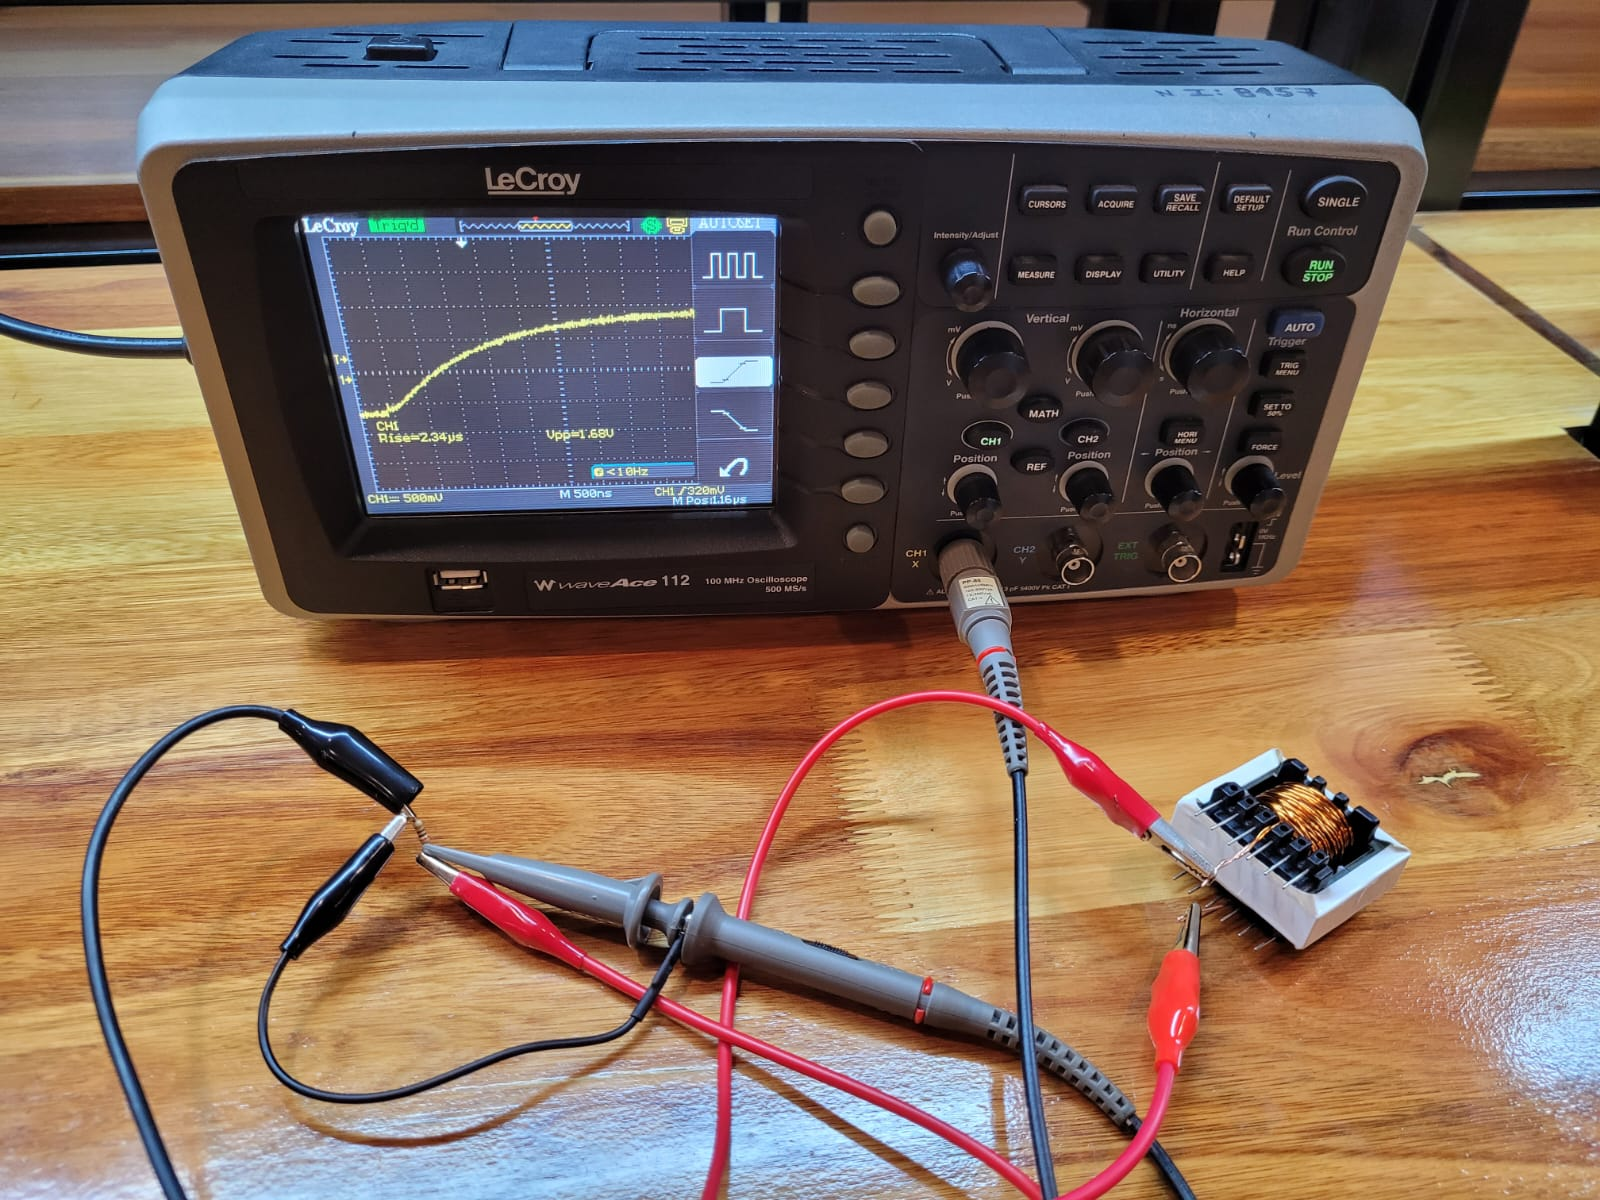
\includegraphics[width=0.8\textwidth]{images/osc-inductor-ts.jpeg}
    \caption{Medición de la inductancia mediante el tiempo de subida}
    \label{fig:osc-inductor-ts}
\end{figure}

\end{enumerate}

\subsection{Driver}

La tensión a la salida del generador PWM es uno de los parámetros de diseño del driver.

$$ V_{drv}=8V $$

La frecuencia de conmutación es: 

$$ f_{drv}=125kHz $$

%3) Carga total del terminal \textit{gate}: Qc

Una de las principales pérdidas de potencia en los transistores MOSFET son las pérdidas por control de puerta o \textit{gate}. 
El encendido y apagado del MOSFET implica la carga y descarga del capacitor interno, 
el cual recibirá o entregará carga cuando la tensión en el mismo se modifique. 
Se requiere de una cierta carga para cambiar la tensión del terminal \textit{gate} entre $0$ y $V_{drv}$. 
Su valor se obtiene mediante el gráfico de la hoja de datos del IRF840 con los siguientes datos:

\begin{itemize}
    \item Rango: $0-63nC$
    \item $V_{gs}=6V$
    \item $V_{ds}=100V$
\end{itemize}

De forma estimada: 

$$ Q_g=26nC $$

%INSERTAR IMÁGEN DE HOJA DE DATOS IRF840: FIGURA 6 Vgs vs Qg
\begin{figure}[ht]
    \centering
    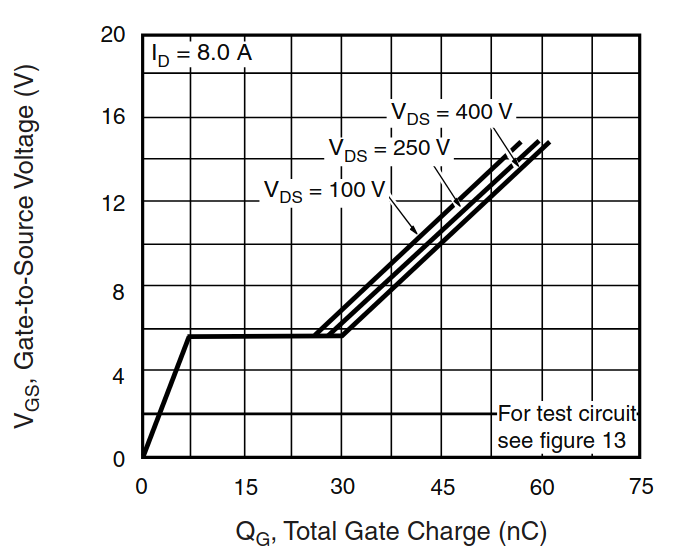
\includegraphics[width=0.8\textwidth]{images/irf840/vgs-vs-qg.png}
    \caption{Curva de tensión entre \textit{gate} y \textit{source} vs. carga del terminal \textit{gate} del IRF840}
    \label{fig:vgs-vs-qg}
\end{figure}

Con este parámetro pueden determinarse la corriente promedio de polarización requerida para controlar el terminal \textit{gate} 
y las pérdidas de potencia de carga de puerta

$$ I_g=Q_g\times f_{drv}=3.25mA $$

$$ P_{gate}=V_{drv}\times Q_g\times f_{drv}=26mW $$

% 4) Delta VC1 y Delta VC2: INSERTAR SÍMBOLOS COMO ANTES

La suma de los ripples en ambos capacitores de acoplamiento aparece en el terminal \textit{gate},
por lo que se elige:

$$ \Delta V_c=0.1\times V_{drv} $$

$$ \Delta V_{c_1}=\Delta V_{c_2}=\frac{\Delta V_c}{2} $$

Para el diodo de rueda libre del secundario se utiliza el mismo diodo que en el convertidor forward, modelo UF4007. 
La tensión directa máxima se obtiene de la hoja de datos: 

$$ V_{dc_2}=1.7V $$

El ciclo de trabajo máximo está definido por el convertidor forward, 

$$ D_{max}=0.5 $$

El valor de la resistencia entre \textit{gate} y \textit{source} se despeja en base a la constante de tiempo deseada en el transitorio de la tensión en el capacitor de acoplamiento.

$$ \tau=50us $$

%INSERTAR CÁLCULO DE RGS

$$ R_{gs}=\frac{\tau}{C_{C_2}} $$

$$ R_{gs}=10k\Omega $$

La inductancia magnetizante $L_m$ se mide con un medidor de inductancias para poder simular el circuito.

$$ L_m=186uH $$

% 9) Cdrv: Capacitor de bypass

% Provee de la corriente necesaria al encenderse. 

% FALTA CÁLCULO
Se agrega un capacitor de bypass entre la alimentación y la tierra del generador PWM para proveer la corriente necesaria en los picos de consumo.

%INSERTAR FÓRMULA DE LA ECUACIÓN 18 JUNTO A LA DESCRIPCIÓN DE SUS parámetros

$$ C_{bypass}=\frac{I_{Q,HI}\frac{D_{max}}{f_{drv}}+Q_G}{\Delta V} $$

Siendo

\begin{itemize}
    \item $I_{Q,HI}$ la corriente de polarización del driver cuando la salida está en alto
    \item $D_{max}$ el ciclo de trabajo máximo
    \item $f_{drv}$ la frecuencia de conmutación
    \item $Q_G$ la carga en el terminal \textit{gate}
\end{itemize}

El capacitor de acoplamiento $C_{C_1}$ se calcula como:

$$ C_{C_1}(D)=\frac{Q_g}{\Delta V_{C_1}}+\frac{(V_{drv}-V_{{dc}_2})\times D}{\Delta V_{C_1}\times R_{gs}\times f_{drv}}+\frac{V_{drv}\times (D^2-D^3)}{\Delta V_{C1}\times 4\times L_m\times f_{drv}^2} $$

La capacidad mínima que asegura permanecer por debajo del ripple de tensión máximo en todas las condiciones de operación 
se puede encontrar determinando el máximo de la expresión anterior:

$$ C_{C_1}=328.3nF $$

Para el capacitor de acoplamiento $C_{C_2}$ se utiliza la siguiente expresión:

$$ C_{C_2}=\frac{Q_g}{\Delta V_{C_2}}+\frac{(V_{drv}-V_{dc_2})D_{max}}{\Delta V_{C_2}R_{gs}f_{drv}} $$

$$ C_{C_2}=71.3nF $$

Finalmente se calcula la resistencia de amortiguamiento en el primario

$$ R_{c_{min}}=2\sqrt{\frac{L_m}{C_{C_1}}}=47.6\Omega $$

Se elige:

$$ R_c=50\Omega $$

El diseño del transformador del driver es similar a un transformador de potencia. 
Para la selección del núcleo, si bien suelen utilizarse núcleos toroidales, en base a la disponibilidad se elige el E30. 
El material del núcleo es N27, cuya alta permeabilidad maximiza el valor de 
la inductancia de magnetización y, en consecuencia, reduce la corriente de magnetización.

El número de vueltas del primario se calcula como: 

$$ N_{1}=\frac {V_{tr}\times t}{\Delta B \times A_{e}} $$

donde $V_{tr}$ es la tensión en el bobinado primario, $t$ es la duración del pulso, 
$\Delta B$ es la variación en el flujo pico a pico durante el tiempo $t$ y $A_{e}$ es la sección transversal equivalente del núcleo. 

\begin{figure}[H]
    \centering
    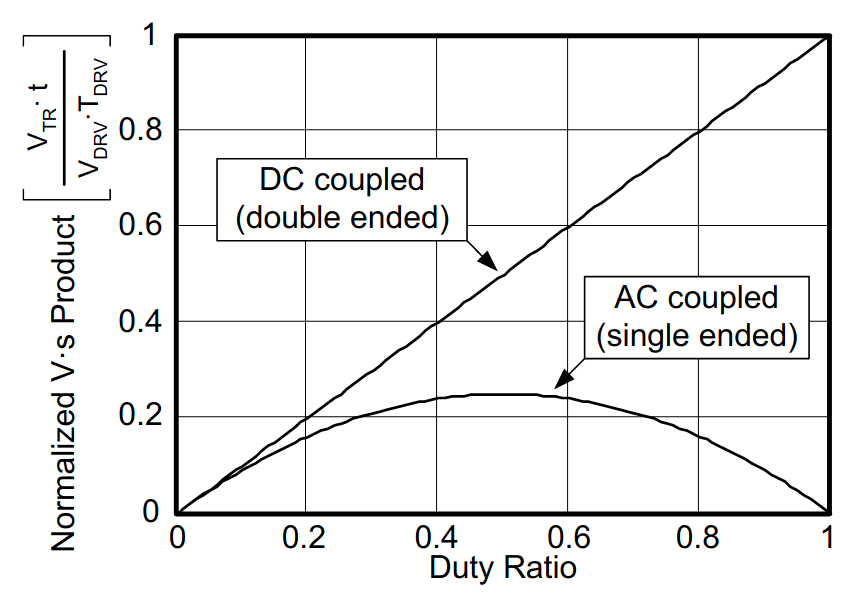
\includegraphics[width=0.8\textwidth]{images/VS-product-vs-duty-ratio.png}
    \caption{Producto volt-segundo en función del ciclo de trabajo.}
    \label{fig:producto-vs}
\end{figure}

Primero se halla el máximo producto volt-segundo del numerador mediante la figura \ref{fig:producto-vs}.
Para un transformador acoplado en alterna, el peor de los casos se da para el ciclo de trabajo máximo $D=0.5$, por lo tanto se obtiene un valor de 0.25. 
Dado que el valor está normalizado, se lo debe multiplicar por la tensión de entrada $V_{drv}=8V$ y por el período de conmutación $T_{drv}=8\mu s$.
De la hoja de datos del núcleo elegido la sección transversal equivalente es $A_{e}=60mm^2$. 
Fijando una variación en el flujo pico a pico de $\Delta B=0.03Wb$ se obtiene: 

$$ N_{1}=\frac {0.25\times 8V \times 8\mu s}{0.03Wb \times 60mm^2}=8.88\simeq 9 $$

Se establece una relación 1:1 para el transformador ya que no se requiere modificar el nivel de tensión.

$$ N_{2}=N_{1}=9 $$

\subsection{Red Snubber}

Se agrega un capacitor de \textit{bypass} de $0.1uF$ para drenar la energía acumulada en la inductancia parásita del MOSFET de lado alto.   
A continuación se describe el procedimiento para el cálculo de los componentes de la red snubber para el MOSFET de lado bajo:

\begin{enumerate}
    \item Con el osciloscopio se mide la frecuencia de la oscilación $f_{r}$ en la tensión del transistor $V_{ds}$. 
    $$ f_{r}=1.25MHz $$ 
    \item Se conecta un capacitor entre \textit{drain} y \textit{source} con una capacidad $C_{p_{0}}$ tal que la frecuencia de la oscilación se reduzca a la mitad. 
    $$ C_{p_{0}}=1.5nF $$
    \item La frecuencia de resonancia en una red LC está dada por la siguiente fórmula:
    $$ f_{r}=\frac{1}{2\pi\sqrt{LC}} $$
    Con la configuración actual: 
    $$ f_{r}=\frac{1}{2\pi\sqrt{L_{p}(C_{p_{2}}+C_{p_{0}})}} $$
    donde $L_{p}$ y $C_{p_2}$ son los componentes parásitos del circuito.
    Para lograr que dicha frecuencia disminuya a la mitad se necesita una capacidad total que sea cuatro veces la capacidad parásita con la que se comenzó.
    Por lo tanto, la capacidad parásita del circuito resulta un tercio de la capacidad agregada:
    $$ C_{p_{2}} = \frac{C_{p_{0}}}{3}=500pF $$
    \item Con la capacidad parásita del circuito y la frecuencia de la oscilación original se puede calcular la inductancia parásita del circuito:
    $$ L_{p}=\frac{1}{(2\pi f_{r})^{2}*C_{p_{2}}}=32.4\mu H $$
    \item La impedancia característica de los elementos parásitos resulta:
    $$ Z_{0}=\sqrt{\frac{L_p}{C_{p_2}}}=255\Omega $$
\item El valor para la resistencia de la red snubber $R_{snb}$ es igual o mayor a la impedancia característica. 
Un valor muy alto puede permitir un pico propio de la oscilación y un valor más bajo permite una corriente más elevada, resultando en un sobrecalentamiento.
$$ R_{snb} \ge Z_{0} $$
El valor elegido fue:
    $$ R_{snb}=340\Omega $$
    \item Se elige una capacitor para la red snubber cuya capacidad sea igual o hasta 4 veces superior a la capacidad parásita del circuito. 
    $$ C_{p_2}\leq C_{snb}\leq 4C_{p_2} $$
    Se optó por un factor 3:
    $$ C_{snb}=C_{p_{0}}=1.5nF $$
    \item Se calcula la potencia disipada en $R_{snb}$ y se utiliza una resistencia cuya potencia máxima sea el doble que la disipada.
    $$ P_{R_{snb}}=C_{snb}V_{in}^2f_{sw}= 243mW $$  
    Se debe utilizar una resistencia de medio watt.
\end{enumerate}

Los componentes utilizados fueron un capacitor cerámico de 1.5nF y dos resistencias en paralelo de $680\Omega$ de un cuarto de watt. 